\documentclass[aspectratio=43,t]{beamer}
%\documentclass[aspectratio=43,t,handout]{beamer}

\usepackage[ansinew]{inputenc}
\usepackage[T1]{fontenc}
\usepackage[english]{babel}
\usepackage{amsmath,amssymb}
\usepackage{graphicx}
\usepackage{listings}
\usepackage[backend=biber,sorting=ydnt,doi=true]{biblatex}


\usepackage{wrapfig}
\usepackage{chngcntr}
\setbeamertemplate{caption}[numbered]
\usepackage{listings}

\usepackage{amssymb}% http://ctan.org/pkg/amssymb
\usepackage{pifont}% http://ctan.org/pkg/pifont
\newcommand{\cmark}{\ding{51}}%
\newcommand{\xmark}{\ding{55}}%

% Themes:
%  - fau:          Default FAU theme
%  - fau-tf:       TechFak FAU theme
%  - fau-tf-hscd:  Co-Design FAU theme
%
% Options:
%  - seal:         FAU seal on title page (default)
	%  - logo:         Beamer logo on all pages
	%  - image:        Cover image on title page
	%  - plain:        Plain title page
	%  - longtitle:    Title page layout for long title
	%  - dark:         Dark version of theme
	\usetheme[seal, longtitle]{fau-tf}
	%\setbeamercovered{transparent}


	\lstset{%
		language=C++,
			tabsize=2,
			basicstyle=\tt\scriptsize,
			keywordstyle=\color{blue},
			commentstyle=\color{green!50!black},
			stringstyle=\color{black},
			% stringstyle=\color{red},
			numbers=left,
			numbersep=0.5em,
			numberstyle=\tt\tiny
	}


\defbibheading{bibliography}{}
\addbibresource[label=primary]{references.bib}
\nocite{*}


% Title, authors, and date
\title[SmartBierdeggl]{SmartBierdeggl}
\subtitle{Projektvorstellung}
\author[Achim Herrmann/Daeubler]{Achim Herrmann/Daeubler}
%TODO Betreuer Prof. J. Teich
% English version
%\institute[Hardware/Software Co-Design]{Hardware/Software Co-Design, University of Erlangen-Nuremberg}
% German version
\institute[Rechnernetze und Kommunikationssysteme]{Rechnernetze und Kommunikationssysteme, Friedrich-Alexander-Universit�t Erlangen-N�rnberg}
\date{October 29, 2015}

\begin{document}
% Title
\frame[plain,c,noframenumbering]{\titlepage}

\begin{frame}{Motivation}
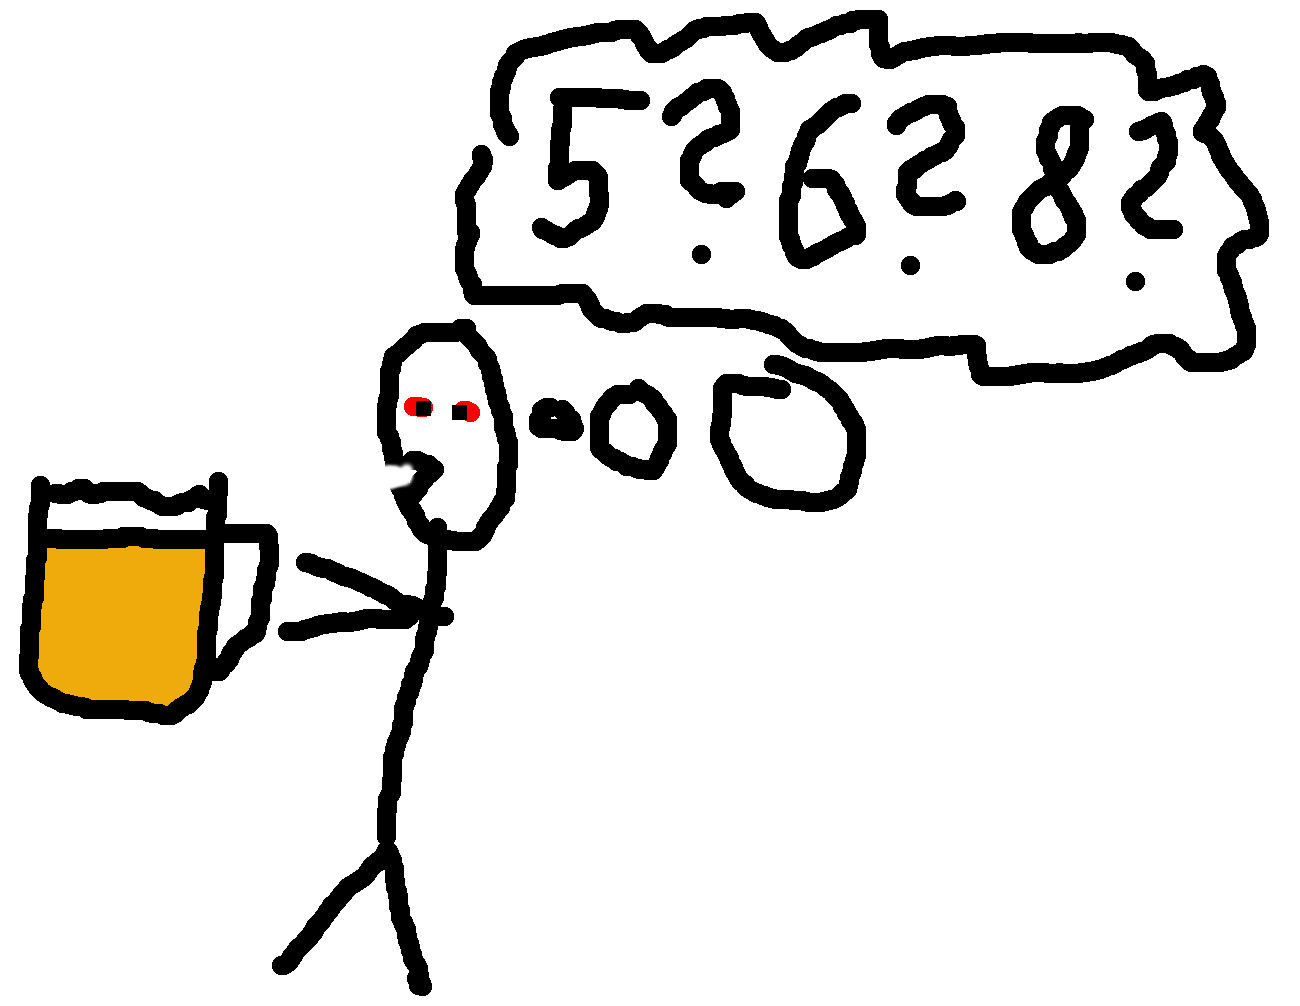
\includegraphics[width=\textwidth]{images/motivation}
\end{frame}

\begin{frame}{Idee}
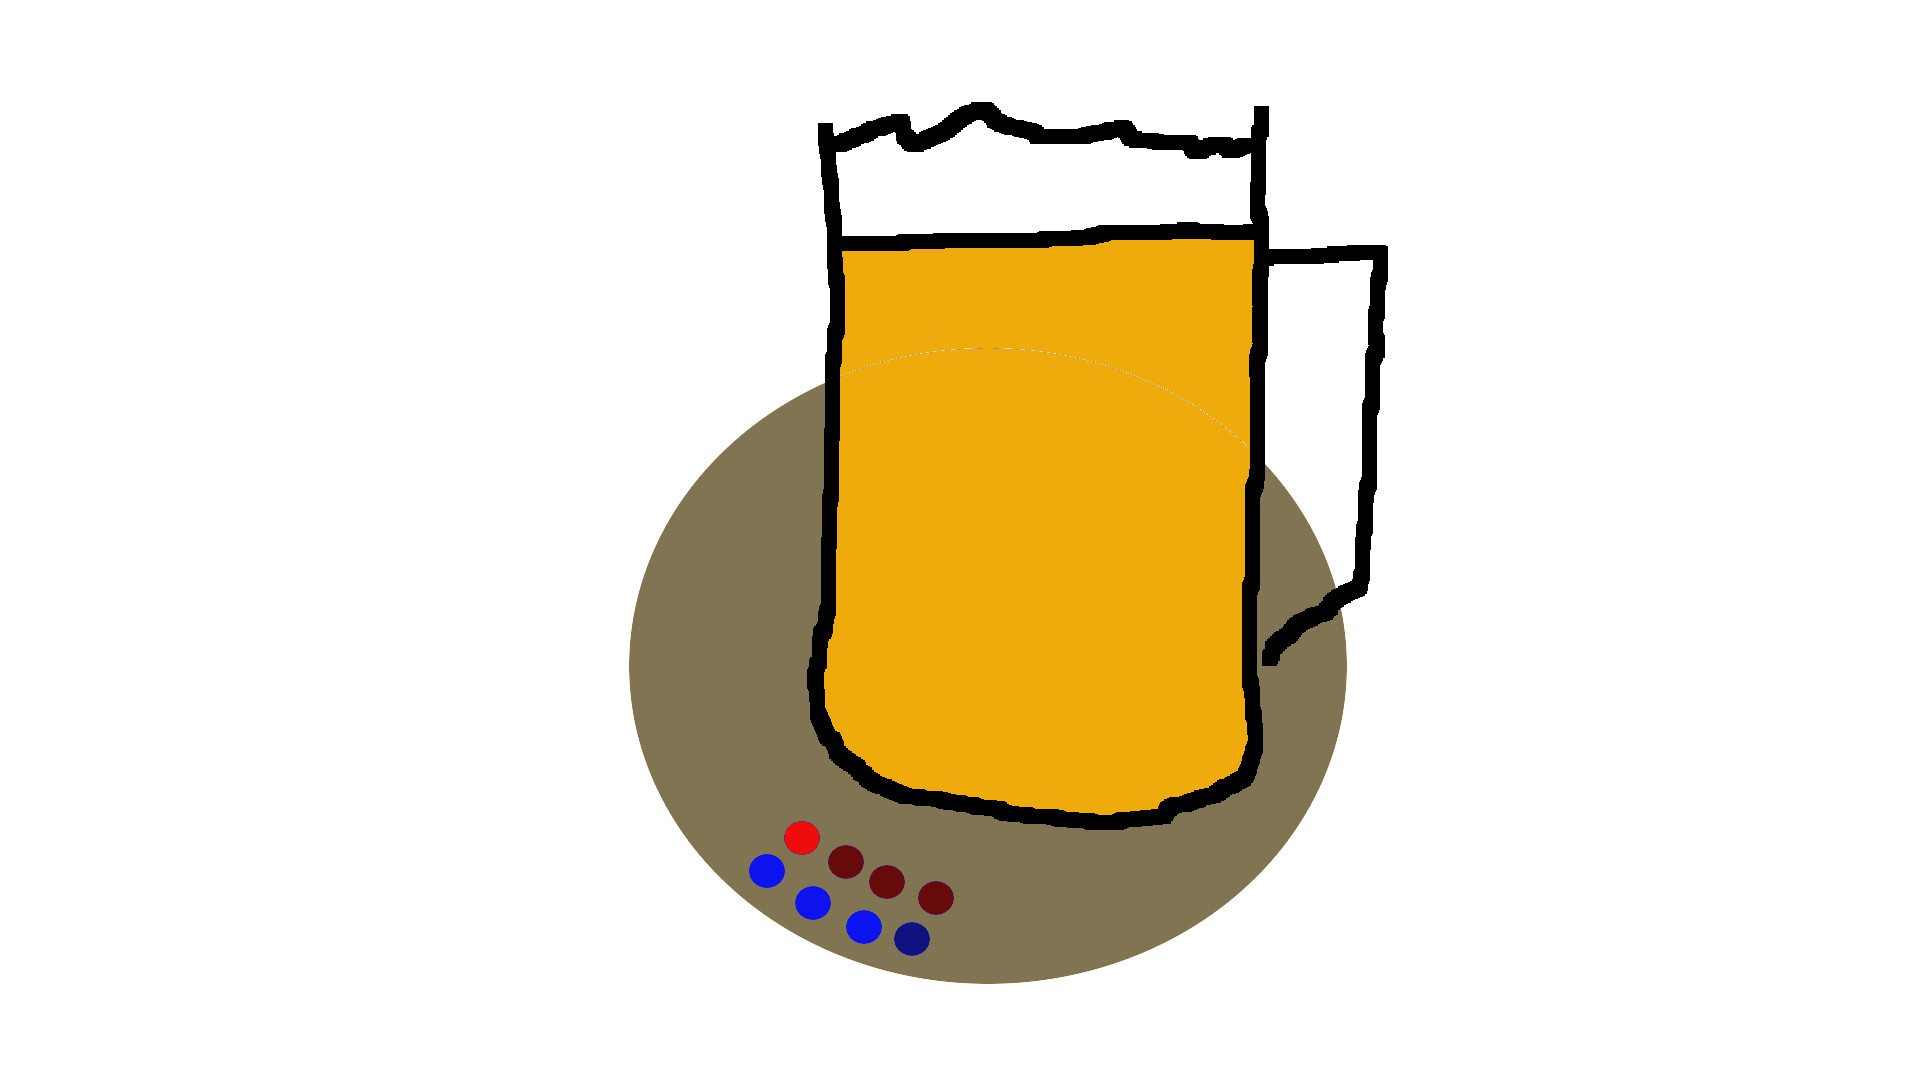
\includegraphics[width=\textwidth]{images/idee}
\end{frame}

\begin{frame}{Aufbau}
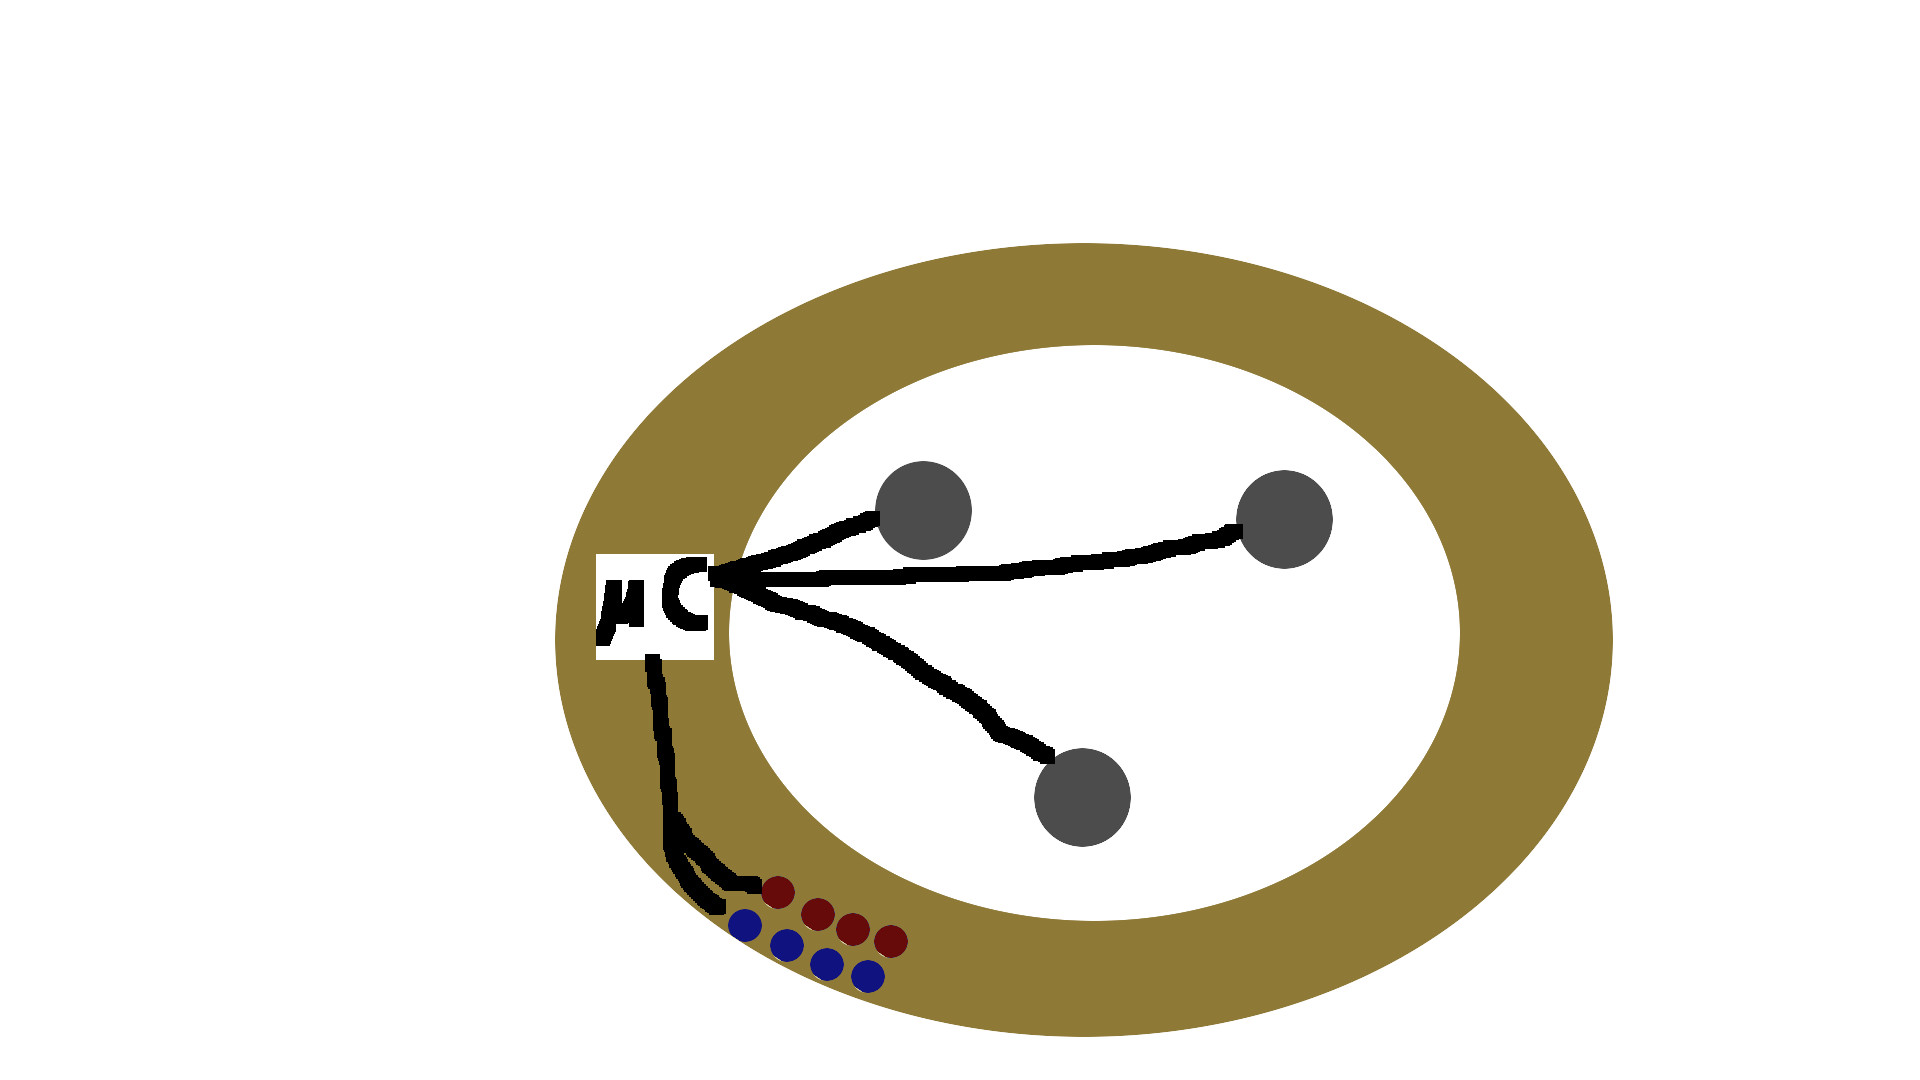
\includegraphics[width=\textwidth]{images/aufbau}
\end{frame}

\begin{frame}{Erweiterungen}
\begin{itemize}
\item Unterscheidung von Getraenken
\item Kommunikation mit Bedienung
\item Anzeige ob man noch fahrtuechtig ist
\end{itemize}
\end{frame}

\begin{frame}{Vision}
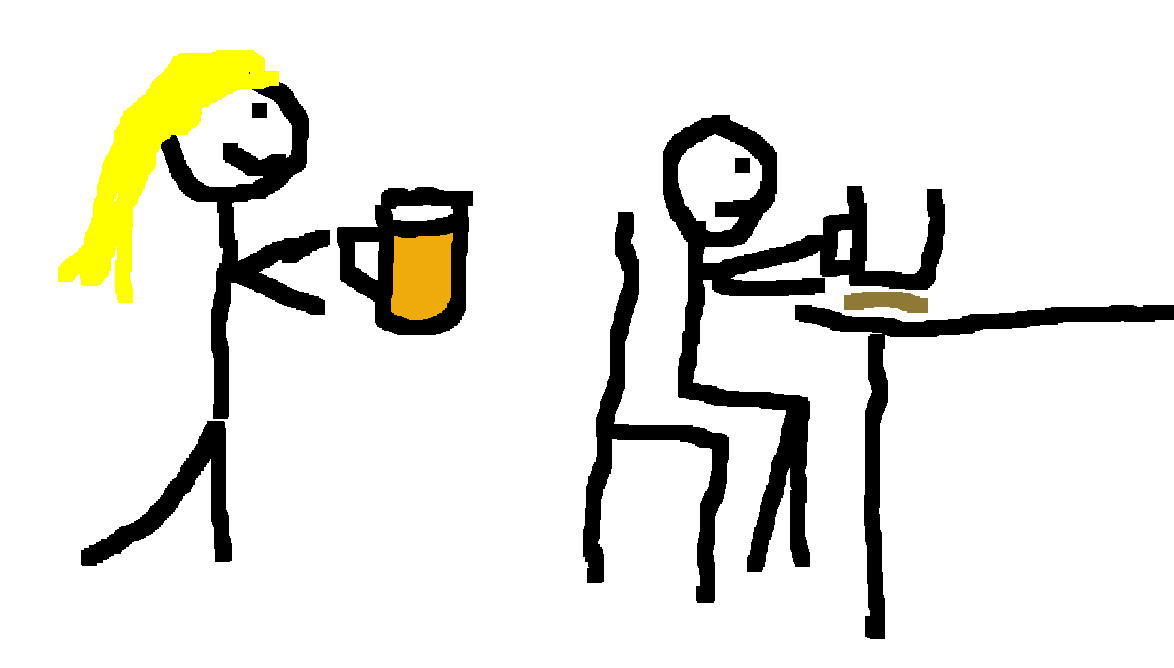
\includegraphics[width=\textwidth]{images/vision}
\end{frame}

%\section{Motivation}
%\begin{frame}{Motivation}
%\begin{itemize}
%	\item Wachsende Zahl mobiler Ger�te mit Android \
%	\visible<2->{\item Auslagerung bestimmter Funktionen von Prozessor auf Hardware}
%	\visible<4->{\item Zusammenspiel zwischen Hardware und Software muss ber�cksichtigt werden}
%	\visible<6->{\item  $\rightarrow$ All-Programmable System-on-a-Chip (APSoC)}
%	\end{itemize}
%
%	\begin{minipage}[b][0.05\textheight][b]{\textwidth}
%	\begin{columns}[T]
%	\begin{column}{0.3\textwidth}  	
%	
%	\includegraphics[scale=0.08]{images/android_smartphone.jpg}
%	\includegraphics[scale=0.07]{images/wear.jpg}\\
%	\includegraphics[scale=0.08]{images/tablet.jpg}
%	\includegraphics[scale=0.08]{images/android-tv.jpg}\\
%	\includegraphics[scale=0.08]{images/Android-Auto.jpg}
%	%TODO Quellen bzw Commen blalbubb
%		\end{column}
%	\begin{column}{0.65\textwidth}
%	
%			\only<2>{\includegraphics[scale=0.43]{tikz/hasoko_ex1.pdf}}
%			\only<3-4>{\includegraphics[scale=0.43]{tikz/hasoko_ex2.pdf}}
%			\only<5->{\includegraphics[scale=0.43]{tikz/hasoko_ex3.pdf}}
%	\end{column}
%	\end{columns}
%	\end{minipage}
%
%	\end{frame}
%
%
%	% Introduction
%	\section{Zynq}
%
%	\begin{frame}{Zynq APSoC}
%
%	\begin{minipage}[0.2\textheight]{\textwidth}
%	\begin{columns}[T]
%	\begin{column}{0.5\textwidth}  
%
%
%	\begin{itemize}
%	\item Dual ARM Cortex-A9 (667MHz - 1GHz)
%\item FPGA   (Artix-7, Kintex-7)
%	\item  ARM Cores $\leftrightarrow$ FPGA Kommunikation
%	\begin{itemize}
%	\item AMBA AXI Ports
%	\begin{itemize}
%	\item 2 General Purpose Master
%	\item 2 General Purpose Slaves
%	\item 4 High Performance Slaves
%	\end{itemize}
%	\item EMIO
%	\item Interrupts
%	\end{itemize}			
%	\end{itemize}
%
%	\end{column}
%	\begin{column}{0.5\textwidth}
%
%%	\includegraphics[scale=0.3]{images/zynq.jpg}
%	\includegraphics[scale=0.6]{tikz/zynq.pdf}
%
%
%
%	\end{column}
%	\end{columns}
%	\end{minipage}
%
%	\end{frame}
%
%	\begin{frame}{Zedboard}
%
%	\begin{minipage}[0.2\textheight]{\textwidth}
%	\begin{columns}[T]
%	\begin{column}{0.25\textwidth}  
%
%
%	\begin{itemize}
%	\item ZC7020
%	\item Artix-7 FPGA
%	\item 667MHz CPU
%	\item 512 MB RAM
%
%	\end{itemize}
%
%	\end{column}
%	\begin{column}{0.75\textwidth}
%	\includegraphics[scale=0.4]{images/zed.jpg}
%	\end{column}
%	\end{columns}
%	\end{minipage}  
%
%	\end{frame}
%
%
%
%	
%	
%	\begin{frame}{Bootvorgang}
%	\begin{minipage}[0.2\textheight]{\textwidth}
%	\begin{columns}[T]
%	\begin{column}{0.5\textwidth}  
%		\begin{itemize}
%	\item On-Chip-ROM
%	\begin{itemize}
%	\item Bei Boot geladen
%	\item Liest Bootdaten von Bootmedium
%	\end{itemize}
%	\item Bootmethoden
%	\begin{itemize}
% 	\item Flash (QSPI, NAND, NOR)
%	\item SD Karte
%	\item JTAG (Slave)
%	\end{itemize}
%	\item FSBL
%	\begin{itemize}
%	\item Konfiguriert FPGA
%	\item L�dt U-Boot
%	\end{itemize}
%\item U-Boot (Universal Boot Loader)
%	\begin{itemize}
%	\item L�dt Linux Kernel
%	\item L�dt Root File System (Android)
%	\item \only<2>{\textcolor{red}}{L�dt Devicetree}
%	\item Bootet Android
%	\end{itemize}
%	\end{itemize}
%
%	\end{column}
%	\begin{column}{0.5\textwidth}
%	\begin{figure}[h!]
%	\centering    
%%	\includegraphics[trim=1cm 2.87cm 1cm 3.2cm, clip=true, scale=0.25]{images/boot.pdf}
%	\only<1>{\includegraphics[clip=true, scale=0.5]{tikz/chart.pdf}}
%	\only<2>{\includegraphics[clip=true, scale=0.5]{tikz/chart_ex.pdf}}
%	%\caption{Boot Vorgang}
%	\end{figure}
%	\end{column}
%	\end{columns}
%	\end{minipage}
%	\end{frame}
%
%	\begin{frame}{Devicetree}
%	\begin{itemize}
%	\item Fr�her: Hardware Details in Kernel codiert
%	\\ $\rightarrow$ Bei Hardware�nderung musste Kernel neu kompiliert werden \pause
%	\item Einf�hrung des Devicetrees
%	\begin{itemize}
%	\item Datenstruktur zur Hardwarebeschreibung
%	\item Separate Boot Datei
%	\item Wird von Bootloader geladen und dem Kernel �bergeben
%	\item $\rightarrow$ Kernel kennt nun die Hardware
%	\end{itemize}
%	\end{itemize}
%	\pause
%	\begin{itemize}
%	\item Device Tree Source (.dts): ASCII Repr�sentation des Devicetrees
%	\item Device Tree Blob (.dtb): Bin�re Form des Devicetrees, f�r Kernel
%	\item Device Tree Compiler (dtc): (De-)Kompilierung von Devicetrees
%	\end{itemize}
%	\end{frame}
%	
%	\begin{frame}{DTS Syntax}
%		\lstinputlisting{images/dt.dts}
%	\end{frame}
%
%	\section{Zwischenstand}
%
%		\begin{frame}{Aufgabenstellung}
%		\begin{block}{Arbeitsschritte}
%		\begin{itemize}
%	\only<1->{\item Einarbeitung} \only<2->{\cmark} 
%	\only<3->{\item Aufsetzen eines Prozessor Subsystems zur Inbetriebnahme essentieller Peripheriekomponenten unter Android (HDMI-Schnittstelle)} \only<5->{\cmark} 
%
%		\only<4-5>{%
%		\begin{itemize}%
%			\item HDMI Controller von Analog Devices
%			\item Linux Kernel von Analog Devices + Xilinx Treiber
%			\item Android 4.1.2 von CambrigeHackers
%		\end{itemize}}
%			
%	
%	\only<6->{\item Entwicklung der DMA Hardware-Software-Schnittstelle durch Implementierung des FPGA-Teils und des Android-Ger�tetreibers} 
%			\only<7-7>{%
%		\begin{itemize}%
%	\item Laplace Filter mit Vivado HLS entwickelt
%	\item Hardware Architektur mit Vivado
%		\end{itemize}}
%	\end{itemize}
%	\end{block}
%
%	\end{frame}	
%	
%
%
%	\begin{frame}{Architektur}
%%	\includegraphics[scale=0.45, angle=270, trim= 4cm 1.5cm 1cm 0cm]{images/filter.pdf}
%	\includegraphics[scale=0.65]{tikz/arch.pdf}
%
%	\end{frame}
%	
%			\begin{frame}{Aufgabenstellung}
%		\begin{block}{Arbeitsschritte}
%		\begin{itemize}
%	\only<1->{\item Einarbeitung} \only<1->{\cmark} 
%	\only<1->{\item Aufsetzen eines Prozessor Subsystems zur Inbetriebnahme essentieller Peripheriekomponenten unter Android (HDMI-Schnittstelle)} \only<1->{\cmark} 
%
%	
%	
%	\only<1->{\item Entwicklung der DMA Hardware-Software-Schnittstelle durch Implementierung des FPGA-Teils und des Android-Ger�tetreibers} \only<2->{\cmark} 
%			\only<2>{%
%		\begin{itemize}%
%	\item Laplace Filter mit Vivado HLS entwickelt %TODO Architektursynthese
%	\item Hardware Architektur mit Vivado
%		\end{itemize}}
%		\only<1-2>{%
%		\begin{itemize}%
%	\item VDMA Treiber von Xilinx
%	\item Eigenen Treiber f�r Hardware Architektur implementiert
%		\end{itemize}}
%	\only<3->{\item Demonstration der Datenkommunikation zwischen Android und FPGA mit Hilfe eines einfachen Beschleunigers }\only<4->{\cmark} 
%	\only<5->{\item Dokumentation }\only<6->{\xmark} 
%	\only<7->{\item Evaluation }\only<8->{\xmark} 
%	\only<9->{\item Pr�fungsarbeit }\only<10->{\xmark} 
%	\end{itemize}
%	\end{block}
%
%	\end{frame}	
%

{ % Questions?
	\setbeamertemplate{footline}{}
	\begin{frame}[c,noframenumbering]
		\begin{center}
	Danke f�r ihre Aufmerksamkeit.\\
	{\bf Noch Fragen?}
	\end{center}
	\end{frame}
}
\end{document}

